\documentclass[10pt,twocolumn,letterpaper]{article}

\usepackage{cvpr}
\usepackage{times}
\usepackage{epsfig}
\usepackage{graphicx}
\usepackage{amsmath}
\usepackage{amssymb}
\usepackage[usenames,dvipsnames]{color}
\usepackage{color}
\usepackage{etoolbox}
\usepackage{listings}
\usepackage{mathtools}
\usepackage{subcaption}
\usepackage{verbatim}
\robustify{\cite}


\definecolor{todo-color}{rgb}{1,0,0}
\newcommand{\todo}[1]{\textnormal{\color{todo-color}{\textbf{#1}}}\unskip}

% Include other packages here, before hyperref.

% If you comment hyperref and then uncomment it, you should delete
% egpaper.aux before re-running latex.  (Or just hit 'q' on the first latex
% run, let it finish, and you should be clear).
\usepackage[breaklinks=true,bookmarks=false]{hyperref}

\cvprfinalcopy % *** Uncomment this line for the final submission

\def\cvprPaperID{****} % *** Enter the CVPR Paper ID here
\def\httilde{\mbox{\tt\raisebox{-.5ex}{\symbol{126}}}}

% Pages are numbered in submission mode, and unnumbered in camera-ready
%\ifcvprfinal\pagestyle{empty}\fi
%\setcounter{page}{4321}
\begin{document}

%%%%%%%%% TITLE
\title{Activation Maps Summarization for CNN Interpretability}

\author{Joana M. F. da Trindade\\
MIT CSAIL\\
{\tt\small jfon@mit.edu}
% For a paper whose authors are all at the same institution,
% omit the following lines up until the closing ``}''.
% Additional authors and addresses can be added with ``\and'',
% just like the second author.
% To save space, use either the email address or home page, not both
\and Matthew Perron\\
MIT CSAIL\\
{\tt\small mperron@mit.edu}
}

\maketitle
%\thispagestyle{empty}

\begin{abstract}
Convolutional Neural Networks (CNNs) are the most effective tools for image classification tasks, yet they remain a black box. Recent work has attempted to improve the ``interpretability'' of CNNs by discovering what each unit in a network learns, one at a time. We propose two method for summarizing whole layers of a CNN, reducing the volume of information to inspect while remaining a powerful method for visually explaining the behavior of these models. We find that our proposed methods allow us to recover perturbations on correctly classified inputs, and find clusters of similar images, visually suggesting the kinds of concepts learned at each layer.
\end{abstract}

\section{Introduction}


\section{Approach}

\begin{itemize}
\item Recap of high level motivation, maybe tie it back to how we differ from related work, e.g., they look at individual units, while we think summaries are enough to recover granularity of concepts recognized in each layer
\item Two main approaches: intra-layer single-image summaries, and intra-layer summary feature vectors \todo{better naming}
\end{itemize}

\subsection{Layer Summaries}

\begin{figure}[b]
\centering
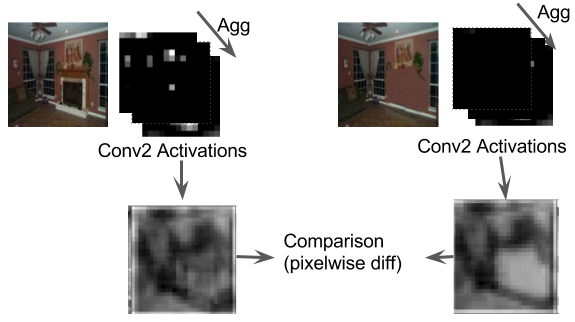
\includegraphics[width=\columnwidth]{figures/layer_summary_fig}
\caption{Generation of Layer Summaries for Comparison with Perturbed Images}

\label{fig:act_im_summary_fig}
\end{figure}

We define a layer summary as an pixel by pixel aggregation over the activations images in a layer of a CNN. For instance, the conv4 layer of Alexnet~\cite{alexnet} contains 256 distinct $14 \times 14$ activation images. We generate an layer summary by aggregating over each pixel across the set of activation images in a layer. Layer summaries are useful for comparing the activations of an image and a perturbed version of the image as in Figure ~\ref{fig:act_im_summary_fig}. We hypothesize that for a perturbed image, where the change in the image does not cause a change in the output class, that the impacts of the change should become less apparent the the summary images of deeper layers of a well behaved network. In a poorly performing network, however, the change will be visible in the summary images of deeper layers.

Different aggregation functions reveal different properties of a set of activation images. For instance, an average has a contribution from all of the input images, but makes it difficult to detect large changes in a single activation image. Whereas, a maximum over the images is sensitive to the changes in a single activation and is unable to detect changes that occur over large sets of activations. We explore the trade-offs of the choice of aggregation in section \todo{add ref to relevant section}.

\subsection{CNN Layer Summaries as Feature Vectors}

\todo{better subsection title because it currently sucks}

To understand how semantic concepts of similar granularity are learned by each individual layer in a network we propose a clustering-based approach.  Specifically, for each labeled image on the validation data set, we extract a feature vector that summarizes how each unit is individually activated by the input image, as show in \ref{fig:vectorization}.  The intuition here is that images which activate similar sets of units from the same layer -- and in similar amounts for each unit -- are likely to contain similar visual concepts.  Therefore, this notion of similarity should be captured by the  feature vector, even if the summarization step loses some information (e.g., exact shape location in the image).

Another way to look at this approach is as a collaborative filtering task -- such as in traditional machine learning -- commonly used in recommendation systems.  Whereas a recommendation system would suggest who to follow or what books to buy based on similar ratings in the past, here our collaborative filtering recommends similar images to a candidate image based on similar amounts of activation on the same units in the layer.  If those units activate for similar concepts in a similar fashion, then the final cluster is cohesive and presents visual evidence of that semantic concept. 

\begin{figure}[t]
\centering
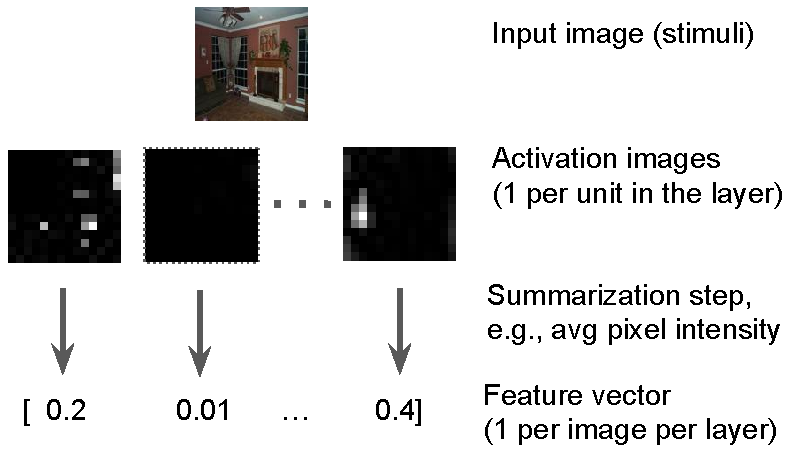
\includegraphics[width=\columnwidth]{figures/vectorization}
\caption{Feature vector obtained for each input image from summarizing its activations on a given CNN layer.}
\label{fig:vectorization}
\end{figure}


\section{Experiments}
\label{s:experiments}

\todo{Describe experiments setup that is common to all tasks: AlexNet \cite{tensorflow} model trained on MiniPlaces dataset \cite{miniplaces}, and MiniPlaces validation images used as stimuli.}

\begin{itemize}
\item Machine and network setup for training (copy-pasta from MiniPlaces report)
\item Questions we want to answer with each set of experiments
\item Subjective evaluation of the results
\end{itemize}

\subsection{Image Clustering by Unit Summaries}

\begin{figure}[!htb]
\centering
  \begin{subfigure}[b]{.24\linewidth}
    \centering
    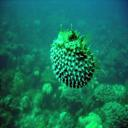
\includegraphics[width=.99\textwidth]{figures/clustering/aquarium}
    \caption{input image}\label{fig:clustering_aquarium_input}
  \end{subfigure}  \\%
  \begin{subfigure}[b]{.99\linewidth}
    \centering
    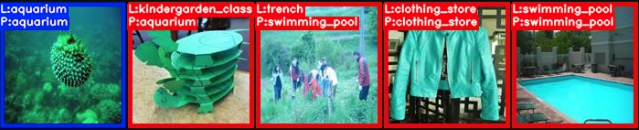
\includegraphics[width=.99\textwidth]{figures/clustering/aquarium_conv1_avg}
    \caption{conv1 cluster (avg activation unit summary)}\label{fig:clustering_aquarium_conv1}
  \end{subfigure}  \\%
  \begin{subfigure}[b]{.99\linewidth}
    \centering
    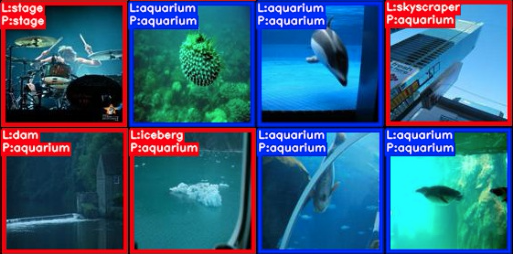
\includegraphics[width=.99\textwidth]{figures/clustering/aquarium_conv4_avg}
    \caption{conv4 cluster (avg activation unit summary)}\label{fig:clustering_aquarium_conv4}
  \end{subfigure}  \\%
  \begin{subfigure}[b]{.99\linewidth}
    \centering
    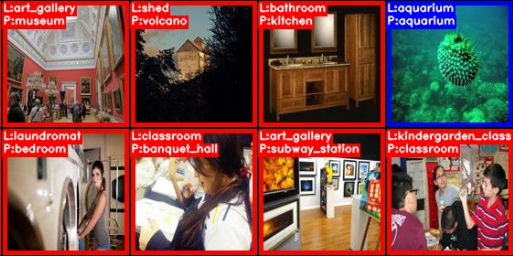
\includegraphics[width=.99\textwidth]{figures/clustering/aquarium_dhash}
    \caption{perceptual image hashing cluster (baseline, no activation information used)}\label{fig:clustering_baseline}
  \end{subfigure}%
  \caption{Figures (b) and (c) show images in the same cluster as the input ``aquarium'' image when the ``average activation'' unit summarization is used to produce each image's feature vector.  Figure (d) displays a qualitative baseline obtained by clustering input images without considering their activations, and instead using the image's perceptual hash difference as distance metric for k-means.}
  \label{fig:aquarium_clusters}
\end{figure}

In this set of experiments, we are trying to determine whether unit summaries capture enough information to suggest what granularity of semantic concept a layer learns to detect.  Recall from Figure~\ref{fig:vectorization} and Section~\ref{ss:approach_feature_vectors} that our working hypothesis is that groups of units activate in similar amounts for input images that describe semantically related scenes, or otherwise contain similar objects.  If that hypothesis is correct, then a feature vector where each dimension is a unit summary when used as basis for clustering should yield clusters with images that are visually similar with respect to concepts learned in that layer.

To validate this hypothesis, our system takes as input the validation data set and, for each image, generates a set of feature vectors that summarize activations for a given layer using one of the following aggregation functions:\\

\noindent {\bf Average activation.} In this feature vector, each activation image -- one per unit for each layer of the CNN, as shown in Figure~\ref{fig:vectorization} -- is summarized as a single value computed as average pixel intensity for all pixels in the activation image for that unit. As expected, this summary loses the location of activated pixels in the original activation image, as well as any shapes present on it, whilst keeping the relative amount of activation normalized by the activation image's size.  
%%In other words, if the CNN when fed with the image of a cat has 40\% of pixels fully activated -- pixel intensity is 1.0 -- and no other pixels activated -- pixel intensity is 0.0 -- in the 2nd unit of convolutional layer 3, then the 2nd dimension of the cat image's \texttt{conv3} feature vector is set to 0.4.

\noindent {\bf Maximum activation.} Here each activation image is summarized as the maximum pixel intensity over all pixels in the activation image, i.e., each dimension in the feature vector is set to the maximum pixel intensity observed for the corresponding activation unit in the layer.  This summary captures very little information, as it loses not only the shape and location of activations in the unit, but also the relative amount of activations.

\noindent {\bf Top 10\% maximum activations.} The value of each dimension in this feature vector is the sum of pixel intensities for the top 10\% most activated pixels in the corresponding unit's activation image.  This aggregation function sits somewhere between the average and maximum summarization steps described above, in that it loses the original shape and location of the activated pixels, while still partially retaining the relative amount of activations for a given input image.

\noindent {\bf Average activations with cutoff.} Each dimension in this feature vector starts out the same way as in the average activation summary vector.  We then set only the top 4 largest dimensions (or average activations) to 1.0 and all other dimensions to 0.  This is the most drastic of summarization strategies we have explored here, in that not only is each activation image transformed into a single value, but a second pass over the vector erases any information regarding how other units activated for the input image under consideration.

In this set of experiments, our prototype generates feature vectors for all 5 convolutional layers -- after ReLu layer -- for all 10,000 validation images in the MiniPlaces dataset.  Each feature vector has as many dimensions as the number of units in the corresponding layer: 96, 256, 384, 256 and 256 respectively for \texttt{conv1} through \texttt{conv5}. This amounts to 50,000 vectors in total (5 per image in the validation set), which are then fed into k-means clustering pipeline -- initial seed using k-means++ -- with euclidean as the distance metric.

We also built a tool that, for a given input image and summarization type, finds the clusters that the image is part of in each of the 5 convolutional layers in our AlexNet model, and visualizes them.  The tool also displays both the original class label and final prediction for each of the images in the cluster.  Finally, the cluster visualizations that the tool produces distinguish between images that are of the same class as the input image, and those that are of a different class.

Figure~\ref{fig:aquarium_clusters} shows a subset of the resulting clusters in which the input image of an aquarium falls into.  Clusters obtained from 3 different configurations of feature vectors for k-means clustering are depicted: when the feature vector is composed of the unit summaries in \texttt{conv1} in AlexNet (Figure~\ref{fig:clustering_aquarium_conv1}), the unit summaries of the \texttt{conv4} in the same network (Figure~\ref{fig:clustering_aquarium_conv4}), and a baseline cluster obtained by image similarity which disregards any information from the CNN (perceptual hash difference as distance measure).  The resulting clusters indicate that, for the input aquarium image, the units that activate on it are those which learn filters based on color transitions, since images that activate the same units in a similar way only share in common large amounts of the same shade of green.

As we go deeper on the layers of the CNN, however, images of the same class are considered similar -- likely because they activate the same units that learn to detect shapes surrounded by bodies of water.  We also get visual explanations for why certain scenes are misclassified, e.g., a skyscraper image turns up in the same cluster, likely because the large building in the image is mostly surrounded by sky which the network could have mistaken for water (both have large amounts of shades of blue).  Finally, Figure~\ref{fig:clustering_baseline} shows that the image similarity cluster obtained when no information from the CNN activations is taken into consideration fails to group images in any meaningful way.  We depict here only the resulting cluster for one of a family of perceptual hashing~\cite{phash_benchmark,imagehash} functions, but our experiments showed similar low quality clusters for all other 4 perceptual hashing functions as well.

\begin{figure}[t]
\centering
  \begin{subfigure}[b]{.24\linewidth}
    \centering
    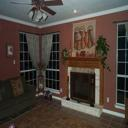
\includegraphics[width=.99\textwidth]{figures/clustering/living_room}
    \caption{input image}\label{fig:clustering_living_room_input}
  \end{subfigure}  \\%
  \begin{subfigure}[b]{.99\linewidth}
    \centering
    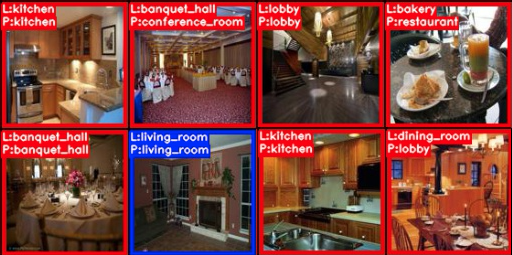
\includegraphics[width=.99\textwidth]{figures/clustering/living_room_conv4_avg}
    \caption{conv4 cluster (avg activation unit summary)}\label{fig:clustering_living_room_conv4}
  \end{subfigure}%
  \caption{Figure (b) shows images in the same cluster as the input ``living room'' scene (a) when the ``average activation'' unit summarization is used to produce each image's feature vector for k-means clustering.}
  \label{fig:living_room_cluster}
\end{figure}

Figure~\ref{fig:living_room_cluster} shows a subset of the images deemed similar to a ``living room'' scene from the validation set in MiniPlaces.  When the input image has higher concentration of complex concepts, unit summaries for deeper layers seem to activate in similar amounts for images that, despite not being from the same class as the input scene, are semantically related. More concretely, ``kitchen'', ``banquet hall'', and ``dining room'' scenes all clustered together with the input ``living room'', likely because these are all indoors images with furniture on them.  This suggests that the same units activate in similar amounts for these visual patterns on \texttt{conv4} of the AlexNet model we used for evaluation.

While it is difficult to generalize our findings without a quantitative measure of cluster ``quality'', we empirically observe from manual qualitative evaluation of randomly sampled clusters that ``average summarization'' seems to work best amongst the aggregations we consider. The rationale for why that is the case is somewhat intuitive: of the aggregation functions above, ``average summarization'' is the only one that correlates with amount of activated pixels originally present in the activation image.


\subsection{Layer Summarization}
\label{sec:exp_layer_summaries}

In this set of experiments we hope to show that we can recover introduced perturbations of input images by examining layer summaries. We hope to see that when classification changes occur, perturbations cause changes through in the summaries of all layers. Whereas when a perturbation does not cause a classification change, a perturbation should become less noticeable in the deeper layers of the network.

We now evaluate qualitatively layer summarization on perturbed images. At a high level, we found that layer summarization is most helpful in validating observations found by our clustering technique. We do this by introducing specialized perturbations to the image, including changing the image hue or removing whole objects with photo manipulation tools. We then compare the summaries for the original image and the perturbed image. the images in all are min-max normalized to best visualize their contents.

Based on our observations from clustering we introduce two kinds of errors to our example images. Namely modifying the hue slightly, as to not change the semantic meaning of the image, and removing whole objects from the image. While we initially attempted to remove objects by replacing them with black regions, we found that this technique added undesirable information, namely large black regions and color to black transitions in the images that may adversely impact classification performance. We eventually decided on manipulating the images by replacing objects patches cloned from nearby areas using a photo manipulation tool. Example of this manipulation is found in the second rows of both both Figure \ref{fig:living_room_ls_fig} and Figure \ref{fig:aquarium_ls_fig}. 

\begin{figure}[tbp]
\centering
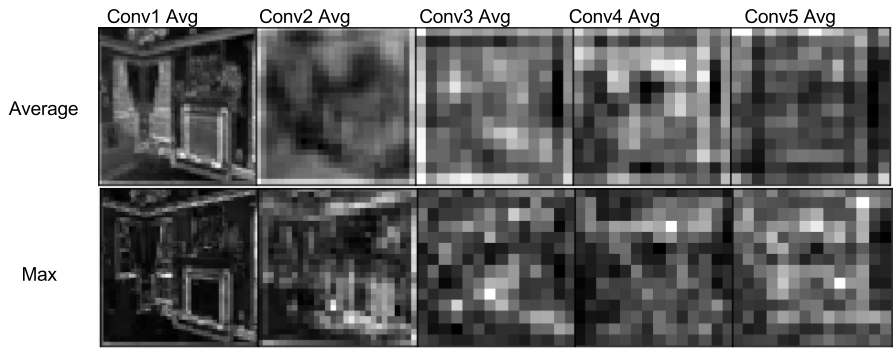
\includegraphics[width=\columnwidth]{figures/layer_summary/avg_vs_max_layer_summary}
\caption{Comparison of Maximum and Average Layer Summary}

\label{fig:avg_vs_max_fig}
\end{figure}

The choice of the aggregation function has a direct impact on the quality and type of information available in a layer summary. We explored two aggregation functions for layer summaries: average and maximum. While the average summary contains contributions from every unit in a layer equally, it is possible that we will not be able to detect large changes in a small number of layers. Alternatively aggregating using a max may miss changes in a large number of layers. In Figure \ref{fig:avg_vs_max_fig} we compare the maximum and average summaries for an example living room image. We found that in both this example and for most of our test images, that the average summary was more useful in finding trends in the summary differences. The maximum images were too noisy to gain meaningful insight into the behavior of the network. There are a wide range of other possible aggregation techniques, including taking the top n\% of activated pixels or a more intelligent scheme based on the weights of the network. We leave this as future work.

\begin{figure}[tbp]
\centering
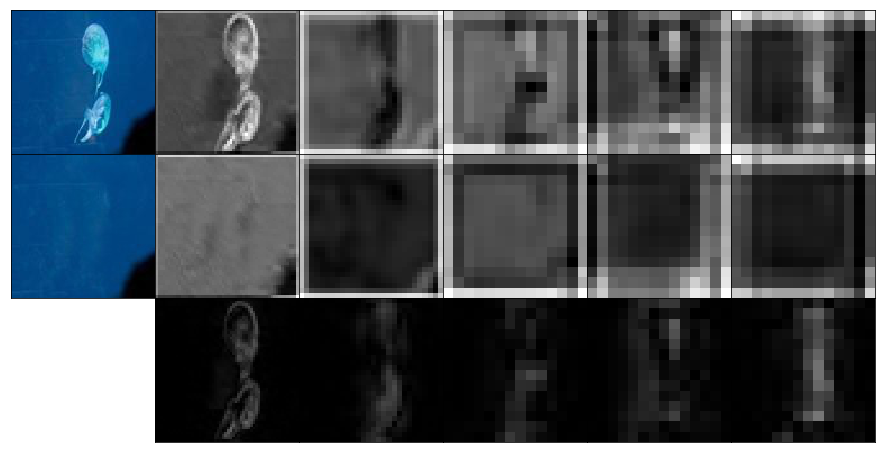
\includegraphics[width=\columnwidth]{figures/layer_summary/aquarium_diff_fig}
\caption{Difference of Layer Summaries in a manipulated image}

\label{fig:aquarium_diff_fig}
\end{figure}

We evaluate the quality of layer summaries by visually comparing the changes in intermediate layers observed by adding perturbations to our images. Comparing the layer-by-layer summaries of an original and a perturbed image reveals changes in the aggregate activations in a layer that may lead to change in the prediction of the network. The process of generating summaries and comparing them for an original image and a perturbed image is demonstrated in figure ~\ref{fig:layer_summary_fig}. Figure ~\ref{fig:aquarium_diff_fig} shows an example of this difference. The top row contains the original image followed by a layer summary of each convolutional layer in our Alexnet model from \texttt{conv1}  to \texttt{conv5}. The second row contains the manipulated image with the fish removed, and its layer summaries. The last row contains the pixel-wise difference of the summaries from the original and manipulated image. While we observe that our manipulation still produces visible effects in the later layers of the network, we reason that the changes in inner pixels were not ultimately important for the classification as the modified image is still classified as an aquarium. 

\begin{figure}[tbp]
\centering
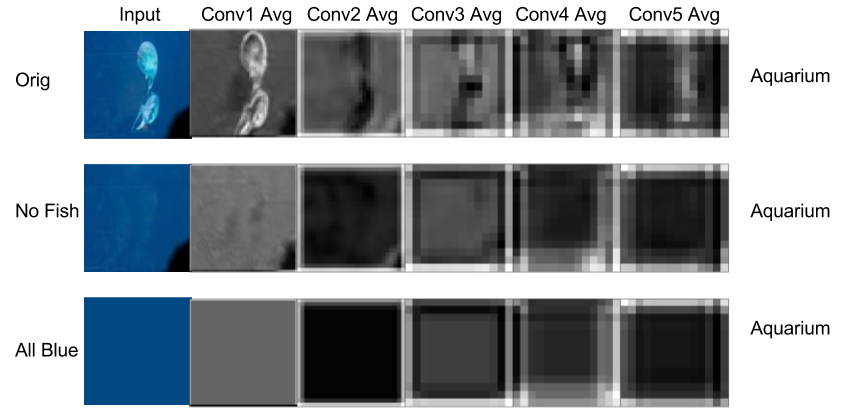
\includegraphics[width=\columnwidth]{figures/layer_summary/aquarium_fig}
\caption{Comparison of Perturbed Aquarium Image with Classification from Alexnet model}

\label{fig:aquarium_ls_fig}
\end{figure}

\begin{figure}[tbp]
\centering
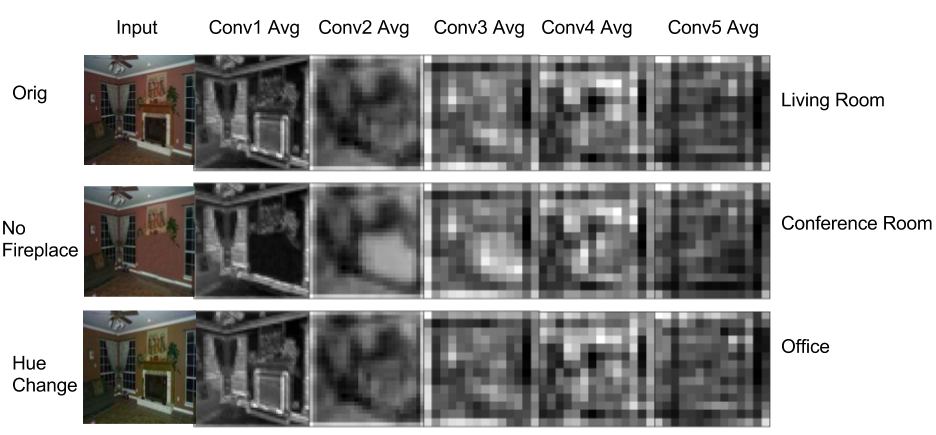
\includegraphics[width=\columnwidth]{figures/layer_summary/living_room_fig}
\caption{Comparison of Perturbed Living Room Image with Classification from Alexnet model}

\label{fig:living_room_ls_fig}
\end{figure}

As the removal of the only recognizable object in the aquarium image did not change the classification result of our network, we deduced that color was one of the most important features for the 'aquarium' class. To further validate this result, we created an artificial image where every pixel is set to the average blue found in the source image. As seen in Figure \ref{fig:aquarium_ls_fig}, none of these changes led to a change in our networks classification, even when all semantic information except color was removed.

We performed similar manipulations on a correctly classified living room image to validate results from clustering indicating depended on detecting objects including furniture in the images. Figure \ref{fig:living_room_ls_fig} shows the original and manipulated images with their respective average layer summary, and the final prediction of our Alexnet model. The first manipulation removes the fireplace, and the second manipulation tweaks the hue of the input image. By comparing the layer summaries for original image and the image without a fireplace, we see that this change has a strong impact on many layers of the network even through \texttt{conv5}. The effect is strongest in the area where the fireplace is removed, and may explain the misclassification. In this case the correct prediction dropped from the networks first rank to it's seventh rank. The second manipulation was a hue change, we found changes of this type much more difficult to detect in layer summary images compared to removing whole objects. 

These experiments may suggest data augmentations that can be added during training to better cover the sets of example on which a given model performs poorly. For instance, we find that some classes are more sensitive to manipulations than others. Some ``aquarium'' images could have nearly all of their semantic content removed while still remaining correctly classified, while some ``living room'' images were more sensitive to these changes. These summarizations were only able to detect some types of perturbations. 

\subsection{Per class histograms}

\todo{Mention MNIST stuff at all? In those we did get some useful information by looking at activation histograms, but that dataset is a lot less complex.}

\begin{itemize}
\item How histogram is derived from layer activations summary
\item Per class correctly classified vs misclassified
\item Mention how it was difficult to extract any meaningful correlations, given that there were little instances of misclassified examples that fall into the same wrong class for a given correct class
\item Mention challenges in terms of dataset diversity, which the clustering approach seems to be robust enough to handle, but a pixel-wise distribution of activations cannot handle (it does fine with simpler datasets such as MNIST)
\end{itemize}
\section{Related Work}
\label{s:related_work}

\noindent {\bf Data visualization for model interpretability.} Approaches that rely on data visualization to increase model interpretability include DrawNet / NetDissect~\cite{netdissect_2017}, which help quantify interpretability of models by measuring and visualizing similarity between known human-interpretable concepts and decisions taken by the CNN model. Another recent example of visualization-based approach is SmoothGrad~\cite{smoothgrad_2017}, which helps recover learned concepts by removing noise from activation images via sequential applications of Gaussian noise.  We believe the latter is complementary to our work, in that our summaries could benefit from the Gaussian filter based denoising step proposed in SmoothGrad, but leave that as future work.

\noindent {\bf Model compression.} In ``Deep Compression'' \cite{deepCompression_2015} the authors introduce Huffman coding compression and model weight quantization to CNN models with the goal of reducing model sizes without loss in model accuracy.  While their work does not share the same goal of model interpretability as in our project, their approach is related to ours in that they show a model's accuracy does not change significantly despite agressive changes to its weights (quantization of learned weights), and to its structure (e.g., pruning of ``unimportant'' connections).  This corroborates with our hypothesis that it is possible to understand what decisions a CNN is taking even if most information on it is summarized.
\section{Conclusion}
\label{s:conclusion}


We proposed two techniques for interpretability of Convolutional Neural Networks: Layer summarization and clustering by unit summarization. We believe these techniques are help augment other tools for better model interpretability. Though both of these techniques are aggressively lossy, we are able to provide insight into how our trained model performs on some groups of images. We find that clustering by unit summarization can find similar images layer-by-layer, and can explain misclassified examples by their similarity to true positive examples in the inner layers of our network. Layer summarization allows us to recover perturbations we introduced, helping to validate our beliefs about the network's behavior. This project suggests future work in finding new summarizations that further improve our results. Less aggressive summarization techniques may reveal more about a network. A next step is to understand how well these techniques work on more complicated, deeper network architectures. 
%\input{contributions}

{\small
\bibliographystyle{ieee}
\bibliography{egbib}
}

\end{document}
